%%%%%%%%%%%%%%%%%%%%%%%%%%%%%%%%%%%%%%%%%
% The Legrand Orange Book
% LaTeX Template
% Version 2.3 (8/8/17)
%
% This template has been downloaded from:
% http://www.LaTeXTemplates.com
%
% Original author:
% Mathias Legrand (legrand.mathias@gmail.com) with modifications by:
% Vel (vel@latextemplates.com)
%
% License:
% CC BY-NC-SA 3.0 (http://creativecommons.org/licenses/by-nc-sa/3.0/)
%
% Compiling this template:
% This template uses biber for its bibliography and makeindex for its index.
% When you first open the template, compile it from the command line with the 
% commands below to make sure your LaTeX distribution is configured correctly:
%
% 1) pdflatex main
% 2) makeindex main.idx -s StyleInd.ist
% 3) biber main
% 4) pdflatex main x 2
%
% After this, when you wish to update the bibliography/index use the appropriate
% command above and make sure to compile with pdflatex several times 
% afterwards to propagate your changes to the document.
%
% This template also uses a number of packages which may need to be
% updated to the newest versions for the template to compile. It is strongly
% recommended you update your LaTeX distribution if you have any
% compilation errors.
%
% Important note:
% Chapter heading images should have a 2:1 width:height ratio,
% e.g. 920px width and 460px height.
%
%	Cities list:
%	New York
%	Bejing
%	London (city)
%	Singapore
%	Dubai
%	Tokyo
%	Los Angeles
%	Frankfurt
%	Brussel
%	Milan
%	Berlin
%
%%%%%%%%%%%%%%%%%%%%%%%%%%%%%%%%%%%%%%%%%

%----------------------------------------------------------------------------------------
%	PACKAGES AND OTHER DOCUMENT CONFIGURATIONS
%----------------------------------------------------------------------------------------

\documentclass[11pt,fleqn]{book} % Default font size and left-justified equations

%----------------------------------------------------------------------------------------

\input{structure} % Insert the commands.tex file which contains the majority of the structure behind the template

\begin{document}

%----------------------------------------------------------------------------------------
%	TITLE PAGE
%----------------------------------------------------------------------------------------

\begingroup
\thispagestyle{empty}
\begin{tikzpicture}[remember picture,overlay]
    \node(background) at (current page.center) {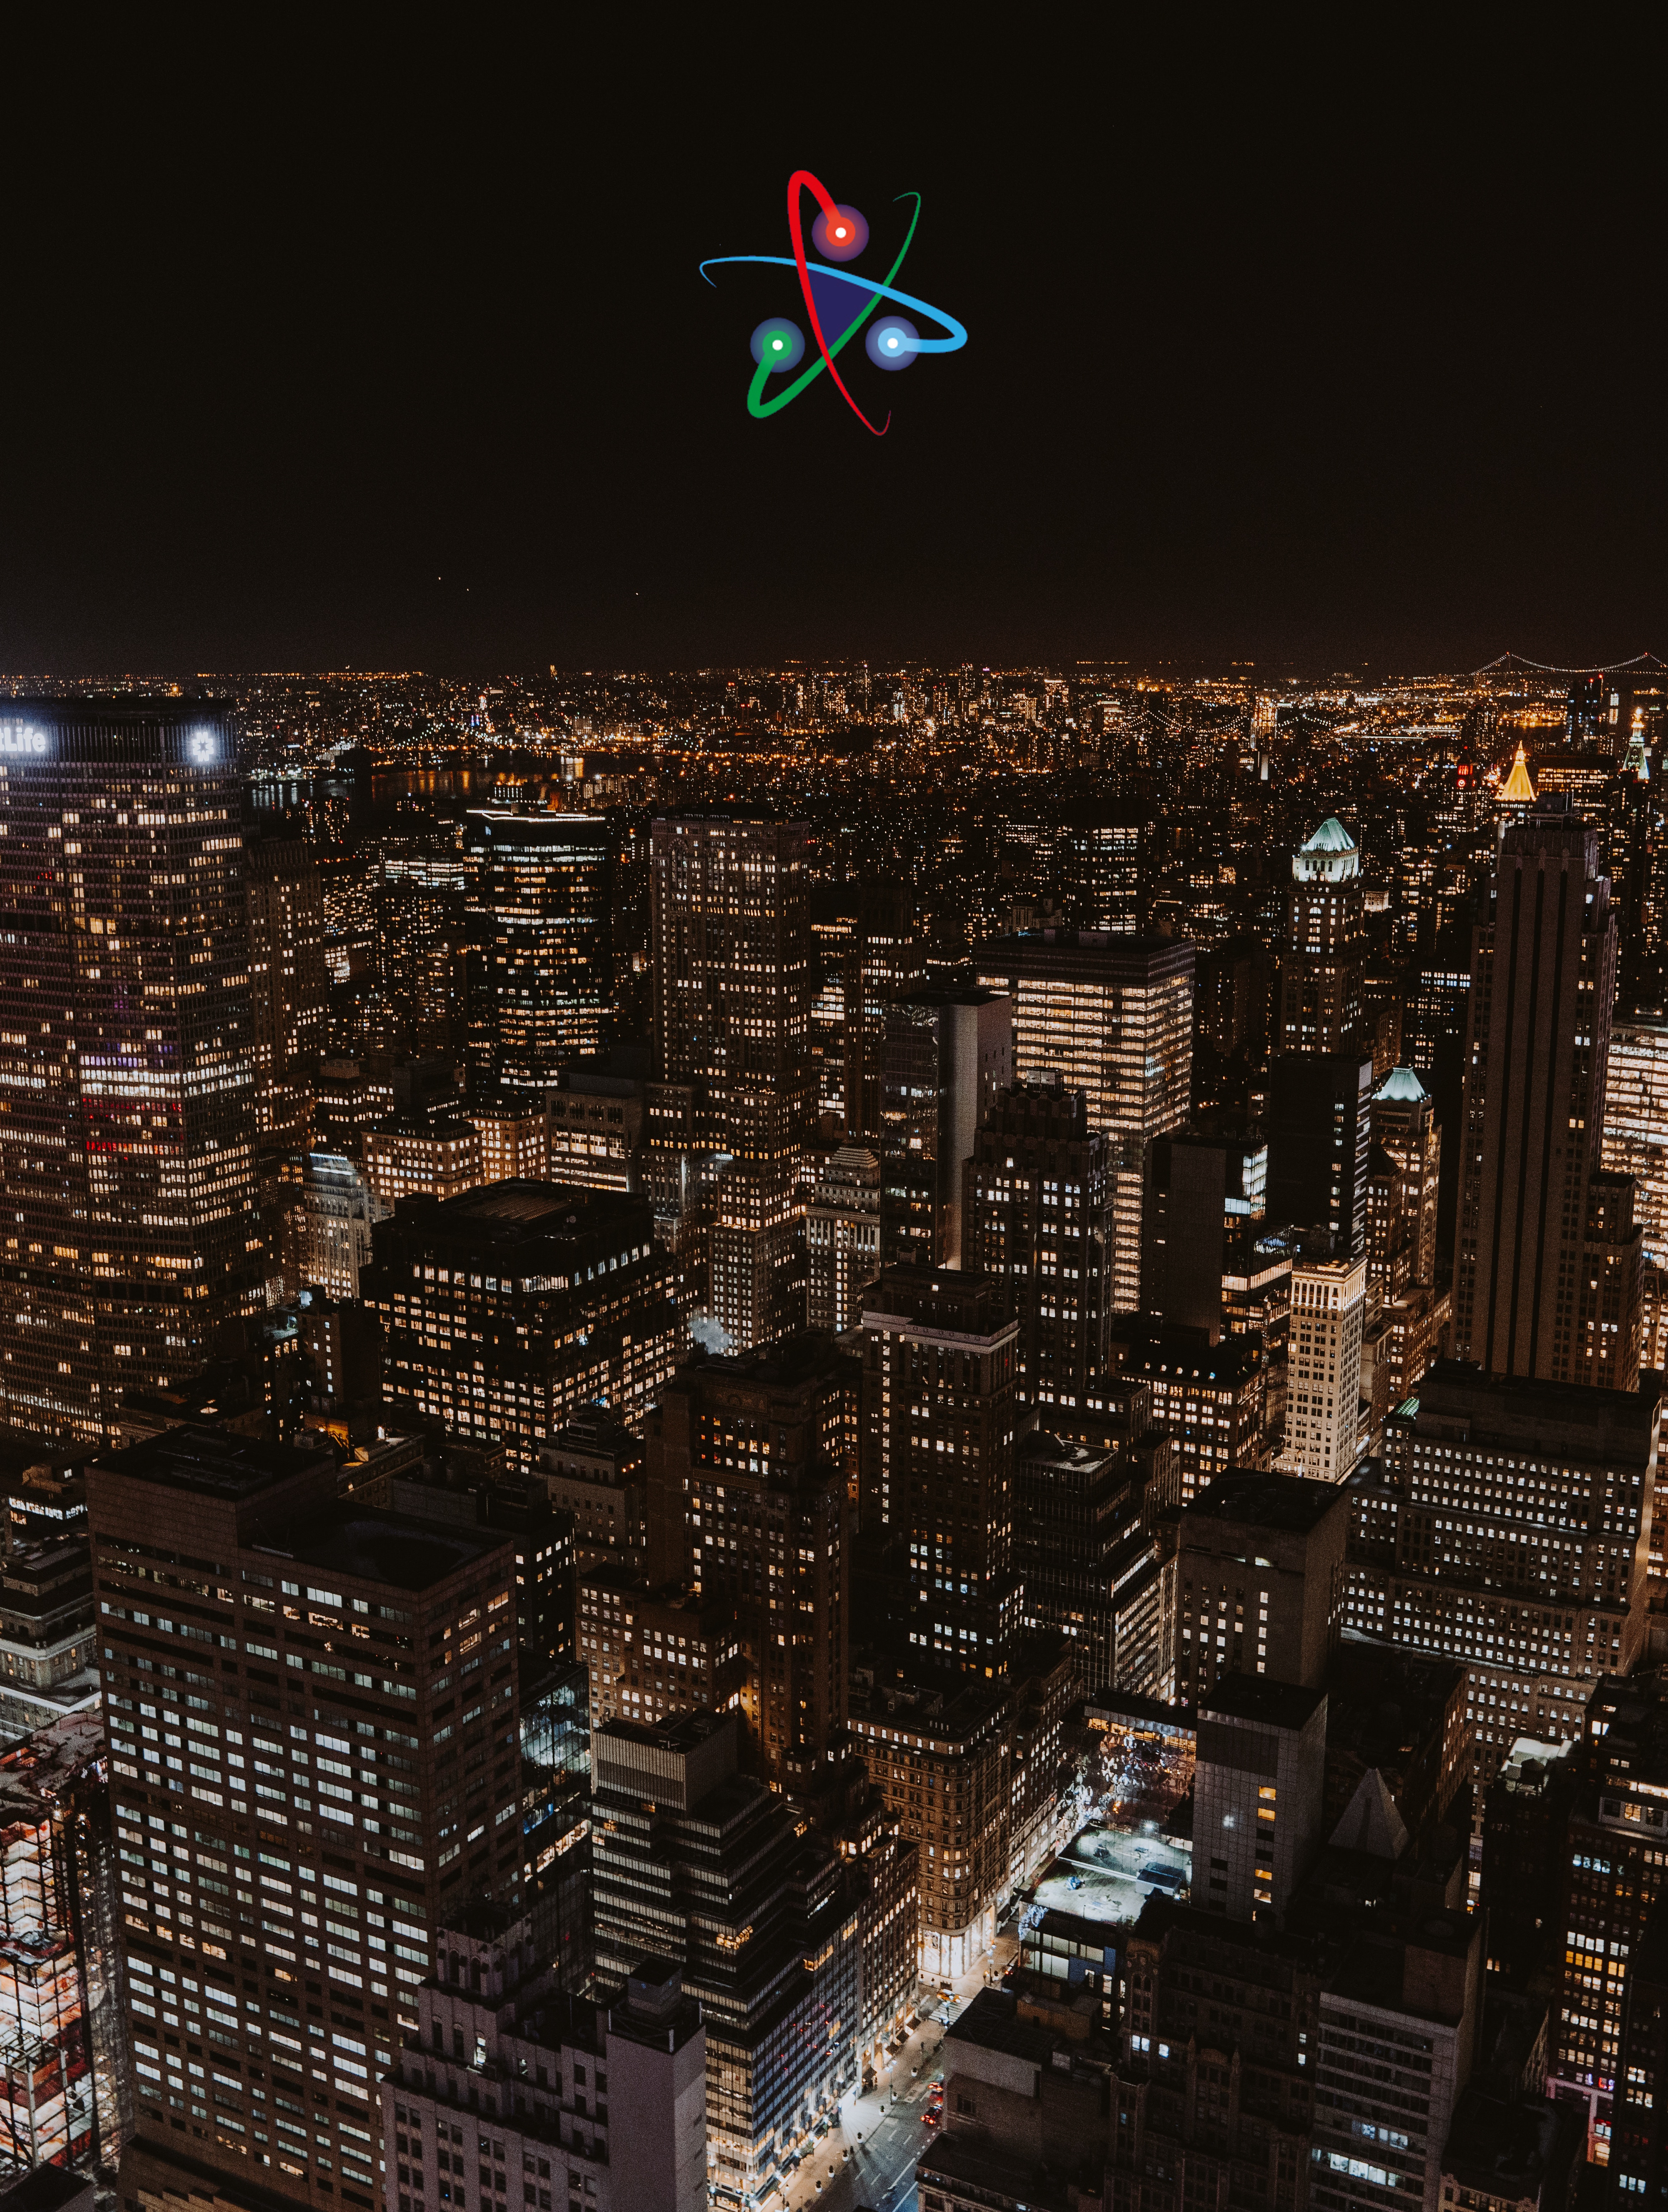
\includegraphics[height=\paperheight]{background}};
	\draw (current page.center) node (title)[fill=airforceblue,fill opacity=0.8,text opacity=1,inner sep=1cm]{\Huge\centering\bfseries\sffamily\parbox[c][][t]{\paperwidth}{\color{silver}\centering RIPAEX\\[15pt]{\Large Crypto Asset Marketplace}\\[20pt]}};
\end{tikzpicture}
\vfill
\vfill
\begin{center}
	\color{silver} \LARGE WHITEPAPER \\
	\color{silver} \large www.ripaex.io
\end{center}
\endgroup

\newpage
\section{Abstract}\index{Abstract}
\textbf{Ripa Exchange is a hybrid-decentralized exchange with a strong focus on lowering the entry level
of opening new exchanges and giving crypto traders safe and secure trading partners to operate on a daily basis.}\\\\
The team of Ripa Exchange believes that, despite the recent developments in the world of
cryptocurrencies, it is still expensive to open, manage and build trust on a newly created exchange not
only for the resources need to run a reliable exchange platform but also for the build of the platform 
itself and to find the liqudity necessary to run a profitable business in the first 3-5 year gap.\\\\
Action is needed and action is needed now. Users are frustrated with unreliable exchanges that run away
with their funds, got hacked or does not sustain the load of a growing industry like this is. Despite
the effort of exchanges managers to offer efficient, reliable, and easy to use platforms to trade entry
prices for building such platforms is in the rage of five-six hundered thousand dollars and that does not 
include personnel cost to give platinum customer support, platform infrastructure and daily expenses for
the business. All of that for then having an decent exchange platform for which you will need to pay an 
external software company to make changes as you request.\\\\
It is the aim of this project to give you an Open Source, efficient, reliable exchange platform and to
give the needed liquidity\footnote{Thank you to the RLSP (Ripa Liquidity Service Provider) technology} to your newly created exchange from day \textbf{one} so you can focus on
finding your customers, give platinum support and comply with all the eterogeneus laws in the industry.
As we want that the customer experience will be the best (the sleekest) as possible while making them safer to trade.\\\\


%----------------------------------------------------------------------------------------
%	COPYRIGHT PAGE
%----------------------------------------------------------------------------------------

%\newpage
%~\vfill
%\thispagestyle{empty}

%\noindent Copyright \copyright\ 2013 John Smith\\ % Copyright notice

%\noindent \textsc{Published by Publisher}\\ % Publisher

%\noindent \textsc{book-website.com}\\ % URL

%\noindent Licensed under the Creative Commons Attribution-NonCommercial 3.0 Unported License (the ``License''). You may not use this file except in compliance with the License. You may obtain a copy of the License at \url{http://creativecommons.org/licenses/by-nc/3.0}. Unless required by applicable law or agreed to in writing, software distributed under the License is distributed on an \textsc{``as is'' basis, without warranties or conditions of any kind}, either express or implied. See the License for the specific language governing permissions and limitations under the License.\\ % License information

%\noindent \textit{First printing, March 2013} % Printing/edition date

%----------------------------------------------------------------------------------------
%	TABLE OF CONTENTS
%----------------------------------------------------------------------------------------

%\usechapterimagefalse % If you don't want to include a chapter image, use this to toggle images off - it can be enabled later with \usechapterimagetrue

\chapterimage{chapter_head_1_Beijing.jpg} % Table of contents heading image

\pagestyle{empty} % No headers

\tableofcontents % Print the table of contents itself

\cleardoublepage % Forces the first chapter to start on an odd page so it's on the right

\pagestyle{fancy} % Print headers again

%----------------------------------------------------------------------------------------
%	PART
%----------------------------------------------------------------------------------------


%\part{Part One}

%----------------------------------------------------------------------------------------
%	CHAPTER 1
%----------------------------------------------------------------------------------------

\chapterimage{chapter_head_2_London.jpg} % Chapter heading image

\chapter{Introduction}

\lipsum[1-3] % Dummy text

%------------------------------------------------

%This statement requires citation \cite{article_key}; this one is more specific \cite[162]{book_key}.

%------------------------------------------------

\section{Key Terminology}\index{Key Terminology}
\begin{description}
	\item[RIPA]: \lipsum[1]
    \item[RIPA Exchange]: \lipsum[2]
    \item[RLSP]: \lipsum[3]
	\item[ARK]: \lipsum[4]
    \item[ACES]: \lipsum[5]
    \item[“,” or “.”]: The Anglo-Saxon use of decimal points and commas to represent numbers has
been chosen for the purposes of this document (except in the accompanying excel
spreadsheets, and the occasional figure or table derived from excel, where continental
numeration has been used). That is to say that a “.” represents a decimal point, and a “,”
distinguishes between multiples of thousands, millions and billions.
[References]: Where sources have not been given, the information has come directly from
RipaEx consortium partners.
    \end{description}

%Lists are useful to present information in a concise and/or ordered way\footnote{Footnote example...}.

\section{Background}\index{Background}
\lipsum[1-2]

There are essentially four phases to the RipaEx project:
\begin{description}
	\item[Information gathering and synthesis (WP2)] This phase recognises the existence of multiple sources of information and experience from
    across Europe concerning the supply chain of biodiesel UCOME. It aims to make the first
    comprehensive analysis of this state of the art to form the basis of the later project phases.    
	\item[The development of tools and resources (WP3)] The second phase takes the results of the first and develops from them a set of tools and
    resources which provide concise and comprehensible guidance to market actors in any
    Member State. With this guidance new biodiesel production facilities can be initiated and
    vehicle fleets converted to biodiesel.    
    \item[The set up of demonstration activities (WP 4-6)] Using the tools and resources developed in WP3, Work packages 4-6 focus on bringing
    collected knowledge and tools into practice. The three work packages reflect three major
    focal points (and target groups) within the supply chain for establishing successful biodiesel
    demonstrations on local scale: production of local biodiesel plants (WP4), distribution
    facilities for biodiesel (WP5), and demand development for fleets (WP6). The demonstration
    phase forms the heart of the OilEx action; WP 2 and 3 are focused on providing
    deliverables (e.g. tools) that enable successful and efficient demonstration activities.    
    \item[Dissemination (WP 7/8) and Project Coordination (WP1)] During the full duration of the project, dissemination activities (WP 7/8) are carried out in
    which results from the individual work packages are disseminated to relevant target groups
    including project partners, OilEx supporters, EC delegates as well as relevant target
    groups. This phase covers a wide range of dissemination techniques, from printed and
    electronic handbooks to workshops and training sessions, ongoing networks, all having the
    ultimate goal of increasing the uptake of biodiesel among public and private transport fleets
    across the EU. An overarching work package is concerned with the management of the
    project from start to finish, ensuring proper coordination, quality assurance and budgetary
    control (WP1).
\end{description}

\section{Summary}\index{Lists!Summary}
\begin{enumerate}
	\item \lipsum[1]
	\item \lipsum[2]
	\item \lipsum[3]
	\item \lipsum[4]
	\item \lipsum[5]
	\item \lipsum[6]
	\item \lipsum[7]
	\item \lipsum[8]
	\item \lipsum[9]
	\item \lipsum[10]
	\item \lipsum[11]
	\item \lipsum[12]
	\item \lipsum[13]
	\item \lipsum[14]
	\item \lipsum[15]
\end{enumerate}


%----------------------------------------------------------------------------------------
%	CHAPTER 2
%----------------------------------------------------------------------------------------

\chapterimage{chapter_head_3_Singapore.jpg} % Chapter heading image

\chapter{In-text Elements}

\section{Theorems}\index{Theorems}

This is an example of theorems.

\subsection{Several equations}\index{Theorems!Several Equations}
This is a theorem consisting of several equations.

\begin{theorem}[Name of the theorem]
	In $E=\mathbb{R}^n$ all norms are equivalent. It has the properties:
	\begin{align}
		 & \big| ||\mathbf{x}|| - ||\mathbf{y}|| \big|\leq || \mathbf{x}- \mathbf{y}||                            \\
		 & ||\sum_{i=1}^n\mathbf{x}_i||\leq \sum_{i=1}^n||\mathbf{x}_i||\quad\text{where $n$ is a finite integer}
	\end{align}
\end{theorem}

\subsection{Single Line}\index{Theorems!Single Line}
This is a theorem consisting of just one line.

\begin{theorem}
	A set $\mathcal{D}(G)$ in dense in $L^2(G)$, $|\cdot|_0$.
\end{theorem}

%------------------------------------------------

\section{Definitions}\index{Definitions}

This is an example of a definition. A definition could be mathematical or it could define a concept.

\begin{definition}[Definition name]
	Given a vector space $E$, a norm on $E$ is an application, denoted $||\cdot||$, $E$ in $\mathbb{R}^+=[0,+\infty[$ such that:
	\begin{align}
		 & ||\mathbf{x}||=0\ \Rightarrow\ \mathbf{x}=\mathbf{0}        \\
		 & ||\lambda \mathbf{x}||=|\lambda|\cdot ||\mathbf{x}||        \\
		 & ||\mathbf{x}+\mathbf{y}||\leq ||\mathbf{x}||+||\mathbf{y}||
	\end{align}
\end{definition}

%------------------------------------------------

\section{Notations}\index{Notations}

\begin{notation}
	Given an open subset $G$ of $\mathbb{R}^n$, the set of functions $\varphi$ are:
	\begin{enumerate}
		\item Bounded support $G$;
		\item Infinitely differentiable;
	\end{enumerate}
	a vector space is denoted by $\mathcal{D}(G)$.
\end{notation}

%------------------------------------------------

\section{Remarks}\index{Remarks}

This is an example of a remark.

\begin{remark}
	The concepts presented here are now in conventional employment in mathematics. Vector spaces are taken over the field $\mathbb{K}=\mathbb{R}$, however, established properties are easily extended to $\mathbb{K}=\mathbb{C}$.
\end{remark}

%------------------------------------------------

\section{Corollaries}\index{Corollaries}

This is an example of a corollary.

\begin{corollary}[Corollary name]
	The concepts presented here are now in conventional employment in mathematics. Vector spaces are taken over the field $\mathbb{K}=\mathbb{R}$, however, established properties are easily extended to $\mathbb{K}=\mathbb{C}$.
\end{corollary}

%------------------------------------------------

\section{Propositions}\index{Propositions}

This is an example of propositions.

\subsection{Several equations}\index{Propositions!Several Equations}

\begin{proposition}[Proposition name]
	It has the properties:
	\begin{align}
		 & \big| ||\mathbf{x}|| - ||\mathbf{y}|| \big|\leq || \mathbf{x}- \mathbf{y}||                            \\
		 & ||\sum_{i=1}^n\mathbf{x}_i||\leq \sum_{i=1}^n||\mathbf{x}_i||\quad\text{where $n$ is a finite integer}
	\end{align}
\end{proposition}

\subsection{Single Line}\index{Propositions!Single Line}

\begin{proposition}
	Let $f,g\in L^2(G)$; if $\forall \varphi\in\mathcal{D}(G)$, $(f,\varphi)_0=(g,\varphi)_0$ then $f = g$.
\end{proposition}

%------------------------------------------------

\section{Examples}\index{Examples}

This is an example of examples.

\subsection{Equation and Text}\index{Examples!Equation and Text}

\begin{example}
	Let $G=\{x\in\mathbb{R}^2:|x|<3\}$ and denoted by: $x^0=(1,1)$; consider the function:
	\begin{equation}
		f(x)=\left\{\begin{aligned}    & \mathrm{e}^{|x|} &  & \text{si $|x-x^0|\leq 1/2$} \\
			 & 0                &  & \text{si $|x-x^0|> 1/2$}\end{aligned}\right.
	\end{equation}
	The function $f$ has bounded support, we can take $A=\{x\in\mathbb{R}^2:|x-x^0|\leq 1/2+\epsilon\}$ for all $\epsilon\in\intoo{0}{5/2-\sqrt{2}}$.
\end{example}

\subsection{Paragraph of Text}\index{Examples!Paragraph of Text}

\begin{example}[Example name]
	\lipsum[2]
\end{example}

%------------------------------------------------

\section{Exercises}\index{Exercises}

This is an example of an exercise.

\begin{exercise}
	This is a good place to ask a question to test learning progress or further cement ideas into students' minds.
\end{exercise}

%------------------------------------------------

\section{Problems}\index{Problems}

\begin{problem}
What is the average airspeed velocity of an unladen swallow?
\end{problem}

%------------------------------------------------

\section{Vocabulary}\index{Vocabulary}

Define a word to improve a students' vocabulary.

\begin{vocabulary}[Word]
	Definition of word.
\end{vocabulary}

%----------------------------------------------------------------------------------------
%	PART
%----------------------------------------------------------------------------------------

%\part{Part Two}

%----------------------------------------------------------------------------------------
%	CHAPTER 3
%----------------------------------------------------------------------------------------

\chapterimage{chapter_head_4_Dubai.jpg} % Chapter heading image

\chapter{Presenting Information}

\section{Table}\index{Table}

\begin{table}[h]
	\centering
	\begin{tabular}{l l l}
		\toprule
		\textbf{Treatments} & \textbf{Response 1} & \textbf{Response 2} \\
		\midrule
		Treatment 1         & 0.0003262           & 0.562               \\
		Treatment 2         & 0.0015681           & 0.910               \\
		Treatment 3         & 0.0009271           & 0.296               \\
		\bottomrule
	\end{tabular}
	\caption{Table caption}
\end{table}

%------------------------------------------------

\section{Figure}\index{Figure}

\begin{figure}[h]
	\centering\includegraphics[scale=0.5]{placeholder}
	\caption{Figure caption}
\end{figure}

%----------------------------------------------------------------------------------------
%	BIBLIOGRAPHY
%----------------------------------------------------------------------------------------

\chapterimage{chapter_head_5_LosAngeles.jpg} % Chapter heading image

\chapter*{Bibliography}
\addcontentsline{toc}{chapter}{\textcolor{darkgoldenrod}{Bibliography}}

%------------------------------------------------

\section*{Articles}
\addcontentsline{toc}{section}{Articles}
\printbibliography[heading=bibempty,type=article]

%------------------------------------------------

\section*{Books}
\addcontentsline{toc}{section}{Books}
\printbibliography[heading=bibempty,type=book]

%----------------------------------------------------------------------------------------
%	INDEX
%----------------------------------------------------------------------------------------

\chapterimage{chapter_head_6_Tokyo.jpg} % Chapter heading image

\cleardoublepage
\phantomsection
\setlength{\columnsep}{0.75cm}
\addcontentsline{toc}{chapter}{\textcolor{darkgoldenrod}{Index}}
\printindex

%----------------------------------------------------------------------------------------

\end{document}
